\documentclass[11pt,reqno]{amsart}

% Add the necessary BibTeX commands
\usepackage{cite}
\bibliographystyle{plain}


%%%%%%%%%%%%%%%%%%%%%%%%%%%%%%%%%%%%%%%%%%%%%%%%%%%
%								Packages									         %
%%%%%%%%%%%%%%%%%%%%%%%%%%%%%%%%%%%%%%%%%%%%%%%%%%%

\usepackage[T1]{fontenc}

\usepackage{amsmath}							
\usepackage{amssymb}
\usepackage{amsthm}
\usepackage{amscd}
\usepackage{amsfonts}
\usepackage{stmaryrd}
\usepackage{algorithm, algorithmic}
\usepackage{ wasysym }
\usepackage{caption}
\usepackage{subcaption}
\usepackage{euler}
\renewcommand{\rmdefault}{pplx}
\usepackage{extarrows}
\usepackage[colorlinks, linktocpage, citecolor = red, linkcolor = blue]{hyperref}
\usepackage{color}
\usepackage{tikz}									
\usepackage{fullpage}
\usepackage[shortlabels]{enumitem}
\usepackage{thmtools}
\usepackage{pythontex}


\linespread{1.1}

%%%%%%%%%%%%%%%%%%%%%%%%%%%%%%%%%%%%%%%%%%%%%%%%%%%
%								Theorems 								         %
%%%%%%%%%%%%%%%%%%%%%%%%%%%%%%%%%%%%%%%%%%%%%%%%%%%

\newtheorem{maintheorem}{Theorem}
\renewcommand*{\themaintheorem}{\Alph{maintheorem}}

\declaretheorem{FundamentalGroup}
\newtheorem{theorem}{Theorem}[section]
\newtheorem{lemma}[theorem]{Lemma}
\newtheorem{proposition}[theorem]{Proposition}
\newtheorem{corollary}[theorem]{Corollary} 
\newtheorem{conjecture}[theorem]{Conjecture} 

\theoremstyle{definition}
\newtheorem{maindefinition}[maintheorem]{Definition}								
\newtheorem{definition}[theorem]{Definition}
\newtheorem{question}[theorem]{Question}
\newtheorem{example}[theorem]{Example}
\newtheorem{construction}[theorem]{Construction}

%\theoremstyle{remark}
\newtheorem{remark}[theorem]{Remark}
\newtheorem{remarks}[theorem]{Remarks}
\newtheorem*{maintheorema}{Theorem \ref{thm:main}}


\renewcommand{\algorithmicrequire}{\textbf{Input:}}
\renewcommand{\algorithmicensure}{\textbf{Output:}}

%%%%%%%%%%%%%%%%%%%%%%%%%%%%%%%%%%%%%%%%%%%%%%%%%%%
%								Operators									         %
%%%%%%%%%%%%%%%%%%%%%%%%%%%%%%%%%%%%%%%%%%%%%%%%%%%


\newcommand{\madeline}[1]{{\color{purple} \sf  Madeline: [#1]}}

\newcommand{\R}{\mathbb{R}}
\newcommand{\C}{\mathbb{F}}
\newcommand{\F}{\mathbb{F}}
\newcommand{\nul}{\mathrm{null}}
\newcommand{\range}{\mathrm{range}}
\newcommand{\spa}{\mathrm{span}}



%%%%%%%%%%%%%%%%%%%%%%%%%%%%%%%%%%%%%%%%%%%%%%%%%%%
%                                                                          Title                                                                             %
%%%%%%%%%%%%%%%%%%%%%%%%%%%%%%%%%%%%%%%%%%%%%%%%%%%

\title{Math 1230: Midterm 1}

\author[M. Carmona]{Marcos Carmona}
\address{Brown University,  Providence, RI 02912}
\email{\href{mailto:marcos_carmona@brown.edu}{marcos\_carmona@brown.edu}}



%%%%%%%%%%%%%%%%%%%%%%%%%%%%%%%%%%%%%%%%%%%%%%%%%%%%%%

\begin{document}


\maketitle
\setcounter{tocdepth}{1}
%\tableofcontents

\section{Problem}
\textbf{Definition:}
    Let $S$ be a set. An $S$-decorated graph is a graph $G$ together with a function $l$ from $V(G)$ to $S$. An isomorphism of $S$-decorated graphs $(G, l), (G', l')$ is an isomorphism $\phi$ from $G$ to $G'$ such that $l(v)$ = $l'(\phi(v))$ for all $v \in V(G)$.

\textbf{Question:}
Let $S$ be a finite set and $n$ an non-negative integer. How many
isomorphism classes of $S$-decorated simple graphs are there with $n$ vertices?

\textbf{My Definitions:}
As my own definition, I'll use the term \textbf{core graph} to denote the undecorated version of an $S$-decorated graph $G$. Similarly, I'll refer to the isomorphism classes of just core graphs for $n$ vertices as \textbf{core isomorphism classes}. 

%%%%%%%%%%%%%%%%%%%%%%%%%%%%%%%%%%%%%%%%%%%%%%%%%%%%%%
\section{Example}
\label{sec:Example}

To get a better understanding of the problem, let's look at a simple example. Let $n = 3$. To get the isomorphism classes of the $S$-decorated graph, we should first look at the isomorphism classes of the core graph. 

\begin{lemma}
    The number of isomorphism classes for an $S$-decorated graph will be greater than or equal to the number of isomorphism classes in the underlying graph.
\end{lemma}

\begin{proof}
    By definition, an isomorphism from $S$-decorated graph $(G, l)$ to $(G', l')$ is an isomorphism from $G$ to $G'$ that satisfies the additional condition that $l(v) = l'(\phi(v)) \: \forall \: v \in V(G)$. This means that if two graphs are in the different isomorphism classes, there is no isomorphism that exists between them, which necessarily implies that there is no isomorphism between them that satisfies the condition. Thus, the lower bound for the number of isomorphism classes of an $S$-decorated graph is the number of isomorphism classes of the core graph, which is the case if $\mid S \mid = 1$.
\end{proof}

By similar logic, for an $S$-decorated isomorphism to be valid, it must be "based" on an isomorphism from $G$ to $G'$, meaning we can look at each isomorphism class independently, and there will be no isomorphism that doesn't fall into one of these overarching categories.

So, let's look at the isomorphism classes of the core graph. For $n = 3$, there are 4 isomorphism classes of graphs. This holds for non-simple graphs as well, since adjacency is the key principle that determines a valid isomorphism after the bijection, so for the rest of the midterm, I'll be essentially dealing with the simple case although it extends for loops and multiple-edges. 

If we break down each isomorphism class, we get the following:

\begin{enumerate}
    \item No edges: We essentially have 3 isolated vertices, which can each be decorated in $|S|$ ways. In this case, all 3 vertices are essentially "equal" since they share every feature apart from possible decoration. What we do know is that for a certain decorated graph with no edges to be isomorphic to another, the number of vertices with a certain decoration from $S$ must be the same. So, with colors being $S$ as an example, if there are two blue vertices and one green vertex, for it to be isomorphic to another graph, that graph must also have two blue vertices and one green vertex. This means that the number of isomorphism classes for this is the amount of triples (unordered and with repetitions) that we can form with elements from $S$, which is $(\mid S \mid + 2) \choose 3$.     

    \item 1 isolated vertex: Essentially, the critical idea to note here is that there is 1 "fixed" vertex, the isolated vertex, that must always map to the corresponding isolated vertex in any isomorphic graph, and 2 vertices that are essentially equal in terms of everything except possible decoration that can map to each other or themselves in a corresponding isomorphic graph.

    As it relates to $S$-decorated isomorphism classes, this means that we have two separate cases to look for. For the fixed vertex $v$, since it is always mapped to the corresponding fixed vertex $v'$ by any isomorphism, but can only be mapped to $v'$ if it has the same decoration, this creates $\mid S \mid$ different isomorphism classes. We now have to multiply the number of isomorphism classes for the two vertices that can map to each other or themselves. This is very similar to the last case, except we now have 2 vertices that can be assigned $\mid S \mid$ decorations, which means we are looking at possible unordered pairs with repition allowed, which is $(\mid S \mid + 1) \choose 2$. So we get a final result of $\mid S \mid \cdot \binom{(\mid S \mid + 1)}{2}$
    \item Two pairs of vertices adjacent: This is identical to the last case, except the fixed vertex isn't isolated, it is the vertex that is connected to both other vertices. We again get the final result of $\mid S \mid \cdot \binom{(\mid S \mid + 1)}{2}$
    \item Maximally Connected: This is the same case as the first, and we know, since isomorphic complements imply isomorphism, that there will be $(\mid S \mid + 2) \choose 3$. 
\end{enumerate}

This gives us a final result of $2|S| \cdot \binom{(\mid S \mid + 1)}{2} + 2\binom{(\mid S \mid + 2)}{3}$



%%%%%%%%%%%%%%%%%%%%%%%%%%%%%%%%%%%%%%%%%%%%%%%%%%%%%%
\section{Literature}
\label{sec:Literature}

For one, it appears the idea of an $S$-decorated graph comes from two more fundamental ideas, the idea of a graph decoration and a labeled graph. A decorated graph generally appears to be a graph where information is encoded into the vertices or edges \cite{lovasz2010limits}, and a labeled graph is just one where the vertices are labeled. From my reading, it appears the decorated graph is very connected to the idea of a graph coloring, where the vertices are colored, which is where the term might have originated from.

The first and only mention of specificly $S$-decorated graphs that I found is in \cite{lovasz2010limits}, which notably is authored partly by Balázs Szegedy who came up in later research on the topic. That being said, in this paper, $S$-decorated graphs were defined more for decorated edges rather than just decorated vertices like the definition in this problem. The paper looked at a topic adjacent to the one we are studying, which is that of graph limits and subgraph density to try and study the structure of $S$-decorated graphs. 

While some of the methods used may be out of the scope of this study, it is worth noting that the methods mentioned in the paper and other papers covering decorations could be useful for studying the number of isomorphism classes for $S$-decorated graphs, namely graph limits and flag algebra, the latter of which is why Balázs Szegedy appeared often in research. 

Luckily, while studying the isomorphism classes of $S$-decorated graphs may require advanced methods to do directly, based on the example I was fairly confident I could reduce the problem to be dependent on the isomorphisms of the core underlying graph and then extend it to $S$-decorated graphs.

Thus, the papers that were most relevant to my exploration, which ended up being algorithmic, were papers on isomorphic comparison algorithms. The main paper were \cite{inproceedings} which covers an efficient solution graph isomorphism problem that I use in my implementation of an algorithm for this problem. 

The graph isomorphism problem is the longstanding problem of finding whether two graphs are isomorphic in polynomial time. While there are conjectures that simplify the problem and allow for efficient solutions, even going back to the 1970s \cite{corneil1970efficient}, the problem is notoriously hard for certain graphs \cite{fortin1996graph}. The problem is still open, but some algorithms have done it really well. The main one that I explored was the one implemented by the NetworkX library that I used for implementation, which is the VF2 algorithm that is not polynomial time for certain difficult examples, but in 2015, László Babai presented a quasi-polynomial time algorithm for the problem which is better.

The VF2 algorithm is actually designed for the subgraph isomorphism problem, which is more difficult, but I'll present a version adapted for the regular graph isomorphic problem. Let $G, G'$ be the two graphs we are testing for isomorphism, with the same number of vertices, otherwise they are obviously not isomorphic. The VF2 algorithm works via depth-first traversal, matching one valid vertex from each at a time (valid superficially being determined by characteristics like degree), until that specific mapping either has no valid choices for remaining $v$ or until it has exhausted every vertex, meaning it is an isomorphism. In the case that it has no valid choices, it backtracks to the last "choice", where more than one valid mapping was possible, and tries the next one. This process is repeated until it finds an isomorphism or exhausts all possibilities, meaning the graphs are not isomorphic \cite{inproceedings}

Additionally, many optimizations are made at the time of implementation of the algorithm, with techniques like pruning to disregard certain branch options, as well as uses of hash tables to quickly compute validity of a mapping based on previous results. While this is not perfect, as mentioned, when optimizations are considered, checking for isomorphisms with VF2 (a key part of the algorithm I state in the next section) is reasonably rapid for most graphs \cite{inproceedings}. 

The trickier problem is producing all of the representatives of each isomorphism class quickly. While algorithms exist, even implemented in NetworkX, to produce all nonisomorphic graphs of a certain type extremely rapidly, like nonisomorphic trees, doing it for all possible graphs of $n$ vertices is much more difficult. No algorithm exists for generating a canonical (standardized representative) graph for all isomorphism classes of a graph in polynomial time. Probably the closest implemented algorithm to it is the geng function in the NAUTY library developed by Brendan McKay for C. 

The core algorithm in NAUTY is an algorithm that finds the automorphism group of a graph, which is the set of all permutations of $V(G)$ that preserve the adjacency relations of the graph, and by extension, can also produce a canonical labeling of the graph \cite{MCKAY201494}. The algorithm itself uses a search method similar to VF2, but with some added notions of partitions as well as other details to produce canonical labeling. The geng function, while optimized and being open to optimizing based on the trick of isomorphism classes of complements being the same, which I use in my algorithm later on, is still fairly slow to be used reasonably. Most algorithms that try to get all representatives get unusable at around 10 vertices, but with the geng function, 11 vertices can be done in 207 seconds, which is fairly reasonable, but it jumps to 9 hours for 12 vertices \cite{timenauty}. 

%%%%%%%%%%%%%%%%%%%%%%%%%%%%%%%%%%%%%%%%%%%%%%%%%%%%%%
\section{Exploration}
\label{sec:Exploration}

For my exploration, there were a few avenues that the example set me down that I thought were interesting and doable so I'll cover those. The first is placing a possible lower and upper bound on the amount, the second is exploring possible recursion or a pattern that could be used to find the number of isomorphism classes, and the third is to try to devise an algorithm to find the number of isomorphism classes, albeit a slow algorithm, and implement in Python using NetworkX.

First, as shown earlier, an isomorphism of $S$-decorated graph must be an isomorphism from the core graph to another core graph, This means that the absolute lower bound for any $S$-decorated graph must be the number of isomorphism classes of the core graph stripped of the decoration, which would be the $|S| = 1$ case. As $|S|$ increases though, the lower bound becomes trickier to find, since it can rapidly increase the amount of classes by just adding a few elements to $S$. But, using the same logic as the example, we see that for a given core isomorphic class, the lowest case scenario is that they're all "equivalent" vertices, meaning they can be mapped to each other. Thus, the absolute lowest case would be that where every vertex is interchangable for every other vertex, which is impossible obviously but gives us a reasonable non-inclusive lower bound of $\binom{|S| + n - 1}{n} \cdot c$, where $c$ is the number of core isomorphism classes.

\begin{proof}
    Suppose we have a core graph isomorphism class with representative $G_c$ with $n$ vertices. Now assume that for this core graph, every vertex is "equal" to every other vertex, meaning that for every vertex $v \in V(G_c)$, there exists an isomorphism $\phi: V(G_c) \rightarrow V(G_c)$ such that $\phi(v) = u$ for all $u \in V(G_c)$. Then, the only condition for assigning decorations to the vertices is that the number of vertices with a certain decoration from $S$ must be the same. 

    Now assume there was a lower number of isomorphism classes for a core graph than $\binom{|S| + n - 1}{n}$, which is the minimum number of nonordered lists of length n with repitions. Then, there must exist two $S$-decorated graphs $S_i, S_j$ with decorations  $l, l'$ that have different unordered lists of decorations that are isomorphic. However, this would mean that there exists some isomorphism $\phi: V(S_i) \rightarrow V(S_j)$ that for some $v, u \in V(G_c)$ with different decorations that maps $\phi(v)$ to $u$. This is a contradiction to the definition of an isomorphism of an $S$-decorated isomorphism, $l(v) \neq l'(\phi(v))$. Thus, the lower bound is $\binom{|S| + n - 1}{n} \cdot c$.
\end{proof}

As for an absolute upper bound, while not inclusive since past $n = 1$ this assumption is not true for every core graph isomorphism class, we could look at the case where no vertices in a given core graph isomorphism class are "equal". This means that you can't map any vertex to another vertex. In this case, we get an upper bound of $|S|^n \cdot c$, since each vertex can be assigned a decoration from $S$ independently. 

\begin{proof}
    Suppose we have a core graph isomorphism class with representative $G_c$ with $n$ vertices. Then, for each vertex $v \in V(G_c)$, we can assign it a decoration from $S$ in $|S|$ ways, giving us $|S|^n$ different possible $S$-decorated graphs. Suppose that for every $S$-decorated graph $S_i$ with core graph $G_c$, there exists no isomorphism $\phi: V(S_i) \rightarrow V(S_j)$ that for no $v, u \in V(G_c)$ maps $\phi(v)$ to $u$. Then, we have $|S|^n$ isomorphism classes for the core graph isomorphism class. 

    Now suppose there does exist an isomorphism $\phi: V(S_i) \rightarrow V(S_j)$ such that for some $v, u \in V(G_c)$ maps $\phi(v)$ to $u$. This means that those two graphs are isomorphic, but no new graph has been added, meaning the number of isomorphism classes for the core graph isomorphism class has necessarily decreased. Thus, the upper bound is $|S|^n \cdot c$, $c$ being the total number of classes.
\end{proof}

As for a recursive pattern, I was unable to find anything meaningful, but I did identify a simple pattern that significantly reduces calculation for the algorithm. This is the simple identification that the number of isomorphism classes inside of a core graph isomorphism class is the same as for the isomorphism class of the complement.

\begin{proof}
    Suppose we have a core graph isomorphism class with representative $G_c$ with $n$ vertices. Suppose the number of $S$-decorated isomorphism classes with core graph $G_n$ was lesser than that of $\bar{G}_n$. Then there exists a decorated graph $S_i$ of $V(G)$ that is isomorphic to some decorated graph $S_j$ with core graph $G_n$, but not with core graph $\bar{G_n}$. However, as we proved in the first problem set, if $S_i$ and $S_j$ are isomorphic, then $\bar{S_i}$ and $\bar{S_j}$ must be isomorphic as well. Since the $S_i$ and $S_j$ have the core graph $G_n$, then their complement must have the core graph $\bar{G_n}$ by the definition of a $S$-decorated graph's core graph we give at the top of the midterm. This is a contradiction, thus they must have the same number of isomorphism classes. For the greater than case, just reverse the argument.
\end{proof}

This effectively reduces the number of calculations in half for the algorithm, since each time you calculate the isomorphism classes within one core isomorphism class, you have calculated them for the complement as well. 

The example gives us a good starting point for an algorithm, as we can follow a similar approach to the example but generalized. We can find the isomorphism classes for the core graph and then for each isomorphism class, then figure out how many isomorphism classes there are for each when you consider the decoration.

\textbf{Algorithm:}
\begin{enumerate}
    \item We partition the graph into all of the core isomorphism classes, and for each we pick an undecorated representative graph.
    \item For each representative graph $G_c$:
    \begin{enumerate}
        \item We initialize with an empty list of marked vertices
        \item Pick an arbitrary vertex $v$ in the graph and form a list of all unmarked vertices that are "equivalent" to $v$ in the representative graph. We define \textbf{equivalence} between vertices $v, u \in V(G_c)$, by the following: $v, u$ are equivalent if there exists an isomorphism $\phi: G_c - v \rightarrow G_c - u$. 
        \item We denote the set of all equivalent vertices to $v$, including $v$, with $\beta$. Using the formula from earlier, as we're trying to find the number of formable unordered lists of length $|\beta|$, we compute the following: $\binom{|S| + |\beta| - 1}{|\beta|}$. We now mark $v$ and every vertex equivalent to $v$ and start the process over from step b until all vertices are marked.
        \item Once they are all marked, we calculate the product of all of the results we got from the previous step, and this is the number of isomorphism classes for the representative core graph isomorphism class. 
    \end{enumerate}
    \item Sum all of these numbers for all of the representative graphs and this is the number of isomorphism classes for $S$-decorated graphs with $n$ vertices.
\end{enumerate}


In other words:

$$\sum^c_{i=1} \prod_{\beta \subset V(G_c)} \binom{|S| + |\beta| - 1}{|\beta|},$$

where $v, x \in \beta$ if $v \equiv x$, $c$ denotes the number of isomorphism classes for the core graph and $G_c$ the representative graph for the core class

To implement this, as mentioned in the literature section, there is no existing library that does this efficiently, thus the efficiency of the algorithm is capped by this algorithm. Additionally, in the worst case for a given representative graph, you must perform approximately $n^2$ isomorphism comparisons on the subgraph induced by removing the two vertices being compared, which also increases the time complexity as there is no algorithm that can do this in polynomial time, although in most cases it is effectively polynomial time.

Unfortunately, in my implementation, I couldn't get the wrapper working for NAUTY, even with a Linux VM, which was very frustrating, so I had to use a similar albeit more limited function in NetworkX called non\_isomorphic\_trees, which generates representatives for all non-isomorphic trees of a given $n$. This has the upside that it is a polynomial time algorithm, so the proposed algorithm can compute extremely high values of $n$ and $|S|$, granted it only produces the number of isomorphism classes where $G$ is a tree. My method should be easily extendable to all classes though given a functioning algorithm to produce all nonisomorphic representative graphs, which I could've written but would've been very slow beyond 9 vertices. The following is the implementation and results for different combinations of $n$ and $S$:

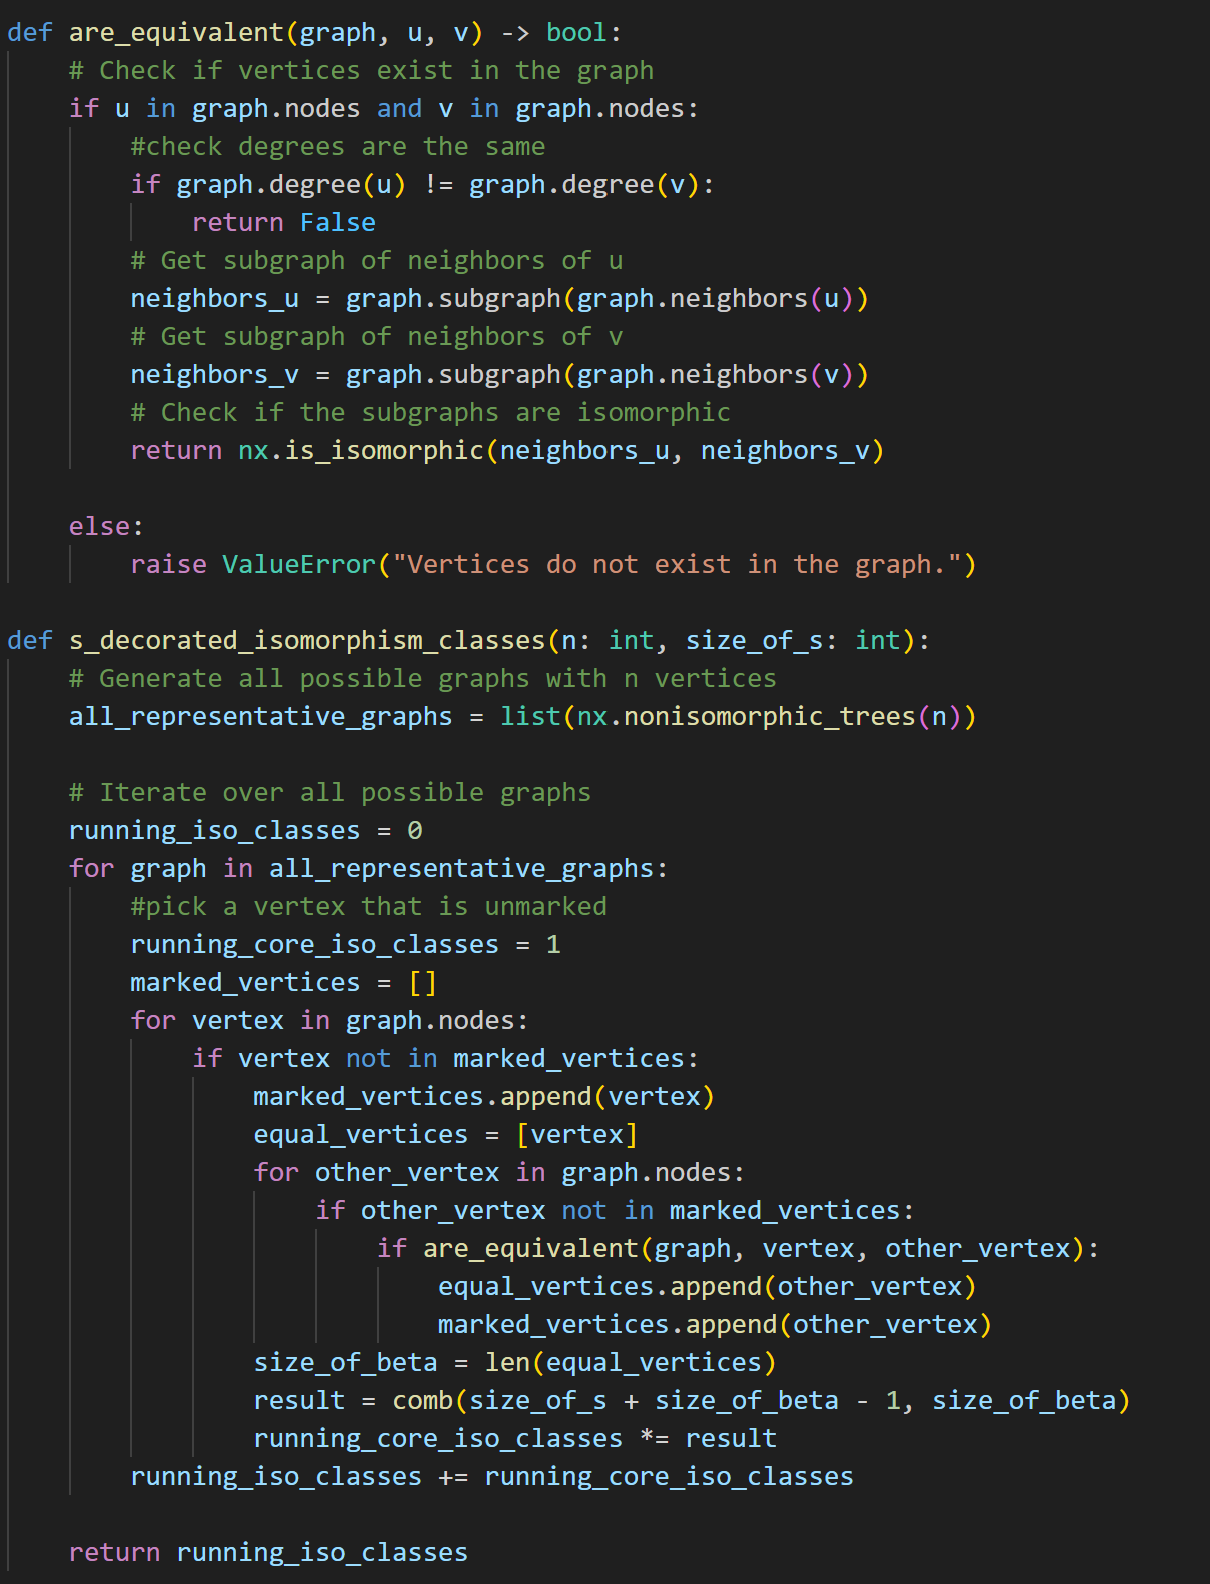
\includegraphics[width=0.5\textwidth]{basefunctions.png}

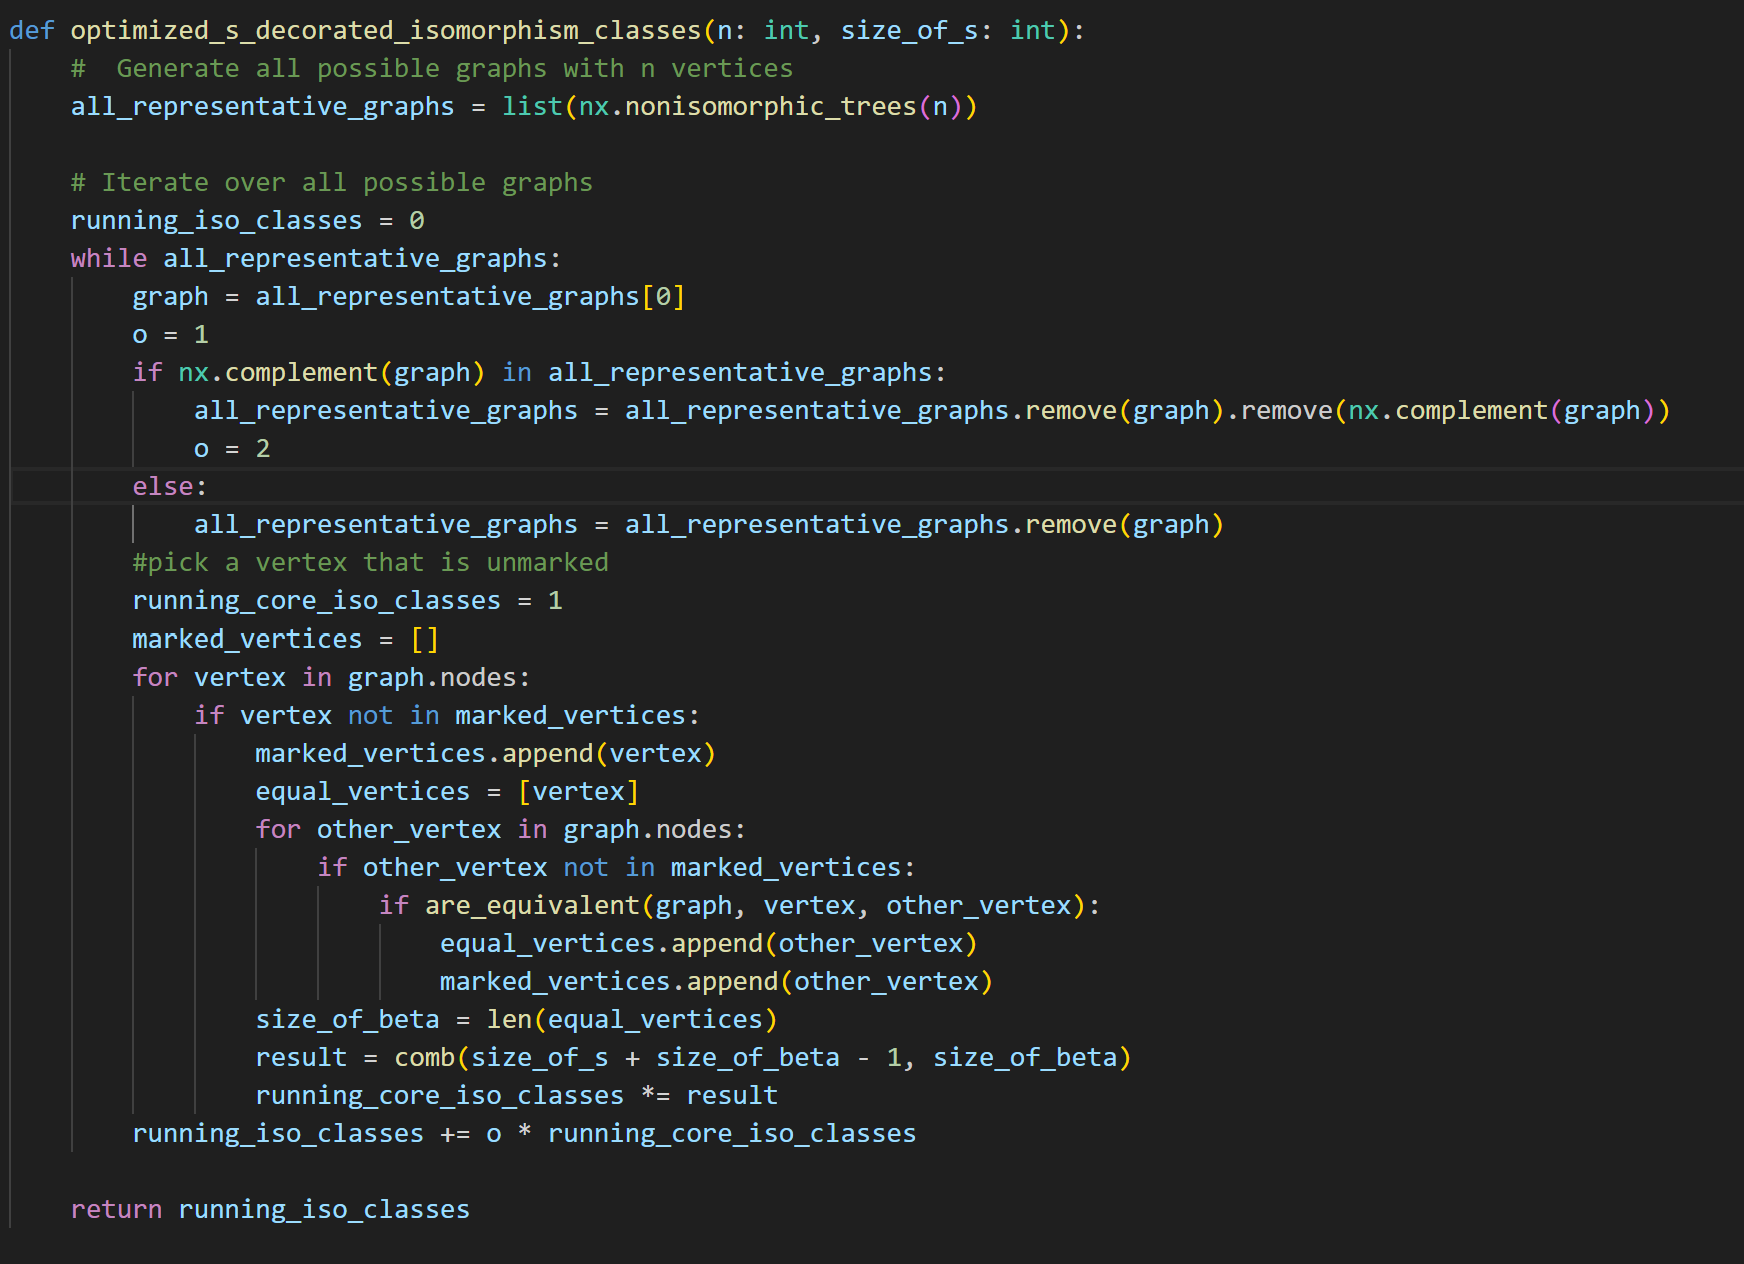
\includegraphics[width=0.8\textwidth]{optimizedfunction.png}

\includegraphics*{Results.png}

\newpage

%%%%%%%%%%%%%%%%%%%%%%%%%%%%%%%%%%%%%%%%%%%%%%%%%%%%%%
\bibliographystyle{abbrv}
\bibliography{Bibliography}

\includegraphics[width=0.7\textwidth]{IMG_0705.jpg}

\end{document}

